% Full instructions available at:
% https://github.com/elauksap/focus-beamertheme

\documentclass{beamer}
\usetheme[numbering=progressbar, nofirafonts]{focus}
\definecolor{main}{RGB}{10,20,43}
\definecolor{background}{RGB}{255,255,255}

\title{MachineLearning and \\DeepLearning courses project}
\subtitle{motion sense dataset proposal}
\author{Mirco De Marchi}
%\titlegraphic{\includegraphics[scale=1.25]{focus-logo.pdf}}
\institute{University of Verona}
\date{28/11/20}

\usepackage{graphicx}
\graphicspath{ {images/} }

% Disable section frame.
%\AtBeginSection[]{} 

\begin{document}

\begin{frame}
\maketitle
\end{frame}

%\begin{frame}
%\frametitle{Contents}
%\tableofcontents
%\end{frame}

% Use starred version (e.g. \section*{Section name})
% to disable (sub)section page.}
\section{Dataset Description}
\begin{frame}{Dataset Description}
 Time-series data generated by accelerometer and gyroscope sensors, collected with an iPhone 6s kept in the participant's front pocket using SensingKit app which collects information.
 \vfill
 A total of 24 participants in a range of gender, age, weight, and height performed 6 activities in 15 trials of different duration in the same environment and conditions: downstairs, upstairs, walking, jogging, sitting, and standing.
 \vfill
The project aim is to predict the activity carried out by a man with a smartphone in his pocket through sensing data and some subject information.
 \vfill
 Reference: \href{https://www.kaggle.com/malekzadeh/motionsense-dataset}{www.kaggle.com/motionsense-dataset};
\end{frame}

\begin{frame}{Features}
Number of features: \textbf{18};

Target feature name: \textbf{\textit{trial type}};

\begin{block}{Participant related features}
	(\textit{subject id}), \textit{weight}, \textit{height}, \textit{age}, \textit{gender}
\end{block}
\begin{block}{Motion related features}
	\textit{attitude.roll}, \textit{attitude.pitch}, \textit{attitude.yaw}, \textit{gravity.x}, \textit{gravity.y}, \textit{gravity.z}, \textit{rotationRate.x}, \textit{rotationRate.y}, \textit{rotationRate.z}, \textit{userAcceleration.x}, \textit{userAcceleration.y}, \textit{userAcceleration.z}, \textit{is long}, \textit{trial type}
\end{block}
\end{frame}

\begin{frame}{Prediction techniques chosen}
Feature selection:
\begin{itemize}
	\item PCA
\end{itemize}
Models:
\begin{itemize}
	\item Bayes decision model (not expected great result)
	\item K-NN with different K and distance metrics
	\item Parzen Window with different kernel and window size
	\item SVM for multiple class 
	\item Markov model on time series 
	\item RNN, CNN, ...
\end{itemize}
\end{frame}

\section{Dataset Analysis}
\begin{frame}{Dimensions and target feature}
Dataset size: \textbf{1412865} entry;

Number of \textit{NULL} values: \textbf{0};
\vfill
The following is the list of classes of \textit{trial type} target feature and the related occurrence of sensing data:
\begin{table} 
	\centering
	\begin{tabular}{rcc}
		Class & Occurrence in dataset \\\hline
		walking & 344288 \\
		sitting & 338778 \\
		standing & 306427 \\
		upstairs & 157285 \\
		jogging & 134231 \\
		downstairs & 131856 \\
	\end{tabular}
\end{table}
\end{frame}

\begin{frame}{Data collection participants}
The following is the number of data collected during the trials of each subject:
\begin{columns}[t, onlytextwidth]
	\column{0.5\textwidth}
	\begin{table} 
		\centering
		\begin{tabular}{rcc}
			Subject & Occurrence\\\hline
			1     & 62312\\
			2     & 62339\\
			3     & 62553\\
			4     & 56066\\
			5     & 52283\\
			6     & 57328\\
			7     & 61276\\
			8     & 60727\\
			9     & 57136\\
			10   &  59796\\
			11   &  59292\\
			12   &  53293\\
		\end{tabular}
	\end{table}
	
	\column{0.5\textwidth}
	\begin{table} 
		\centering
		\begin{tabular}{rcc}
			Subject & Occurrence \\\hline
			13    &  51147\\
			14    &  56487\\
			15    &  59443\\
			16    &  65417\\
			17    &  55539\\
			18    &  62808\\
			19    &  71949\\
			20    &  55153\\
			21    &  68932\\
			22    &  56028\\
			23    &  54556\\
			24    &  51005\\
		\end{tabular}
	\end{table}
\end{columns}
\end{frame}

\begin{frame}{Relation between feature and target 1}
\begin{figure}
	\centering
	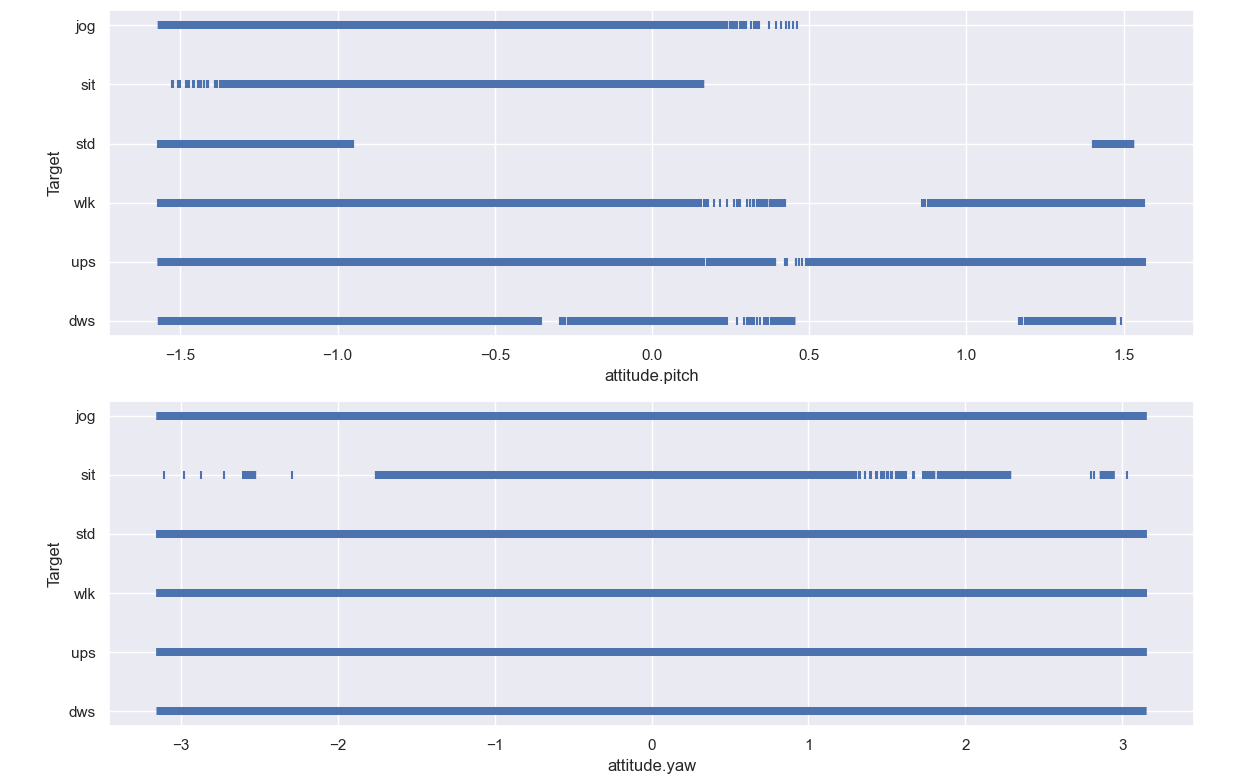
\includegraphics[scale=0.3]{relations1.png}
	\label{fig:relations1}
\end{figure}
\end{frame}

\begin{frame}{Relation between feature and target 2}
\begin{figure}
	\centering
	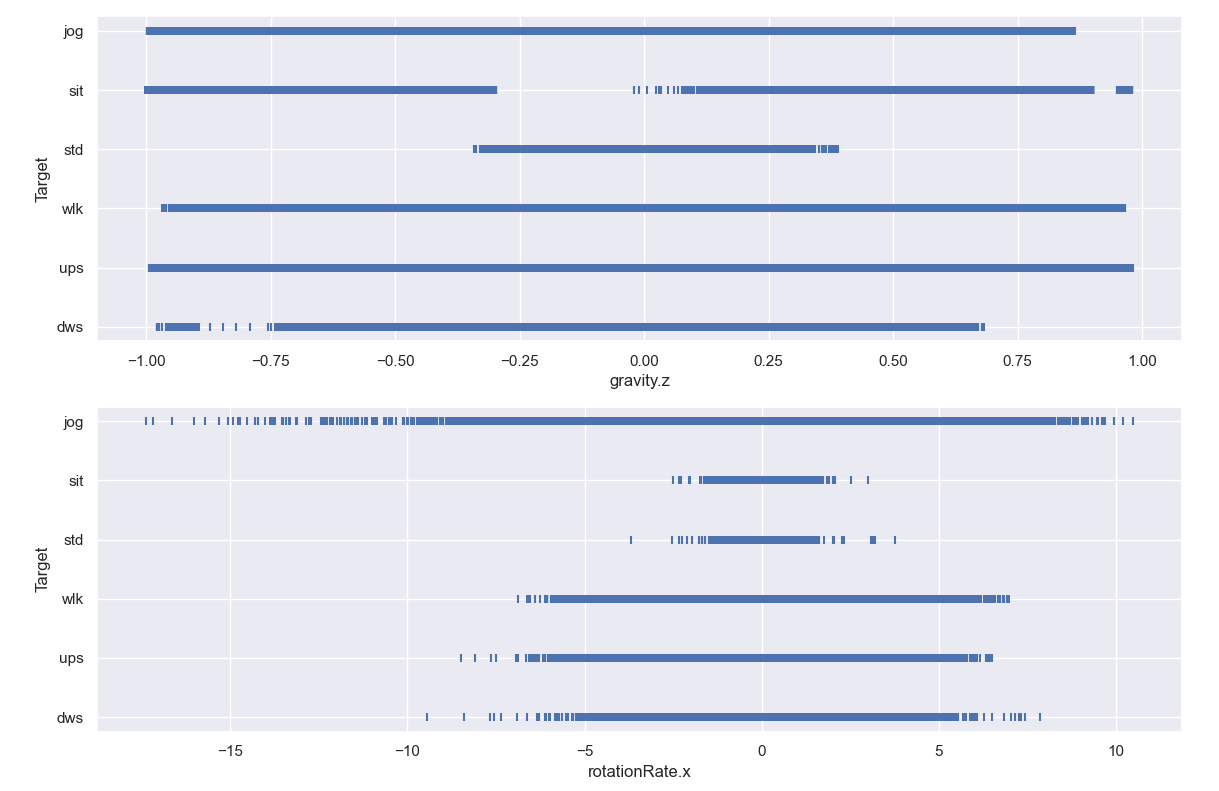
\includegraphics[scale=0.3]{relations2.png}
	\label{fig:relations2}
\end{figure}
\end{frame}

\begin{frame}{Correlation Matrix}
\begin{figure}
	\centering
	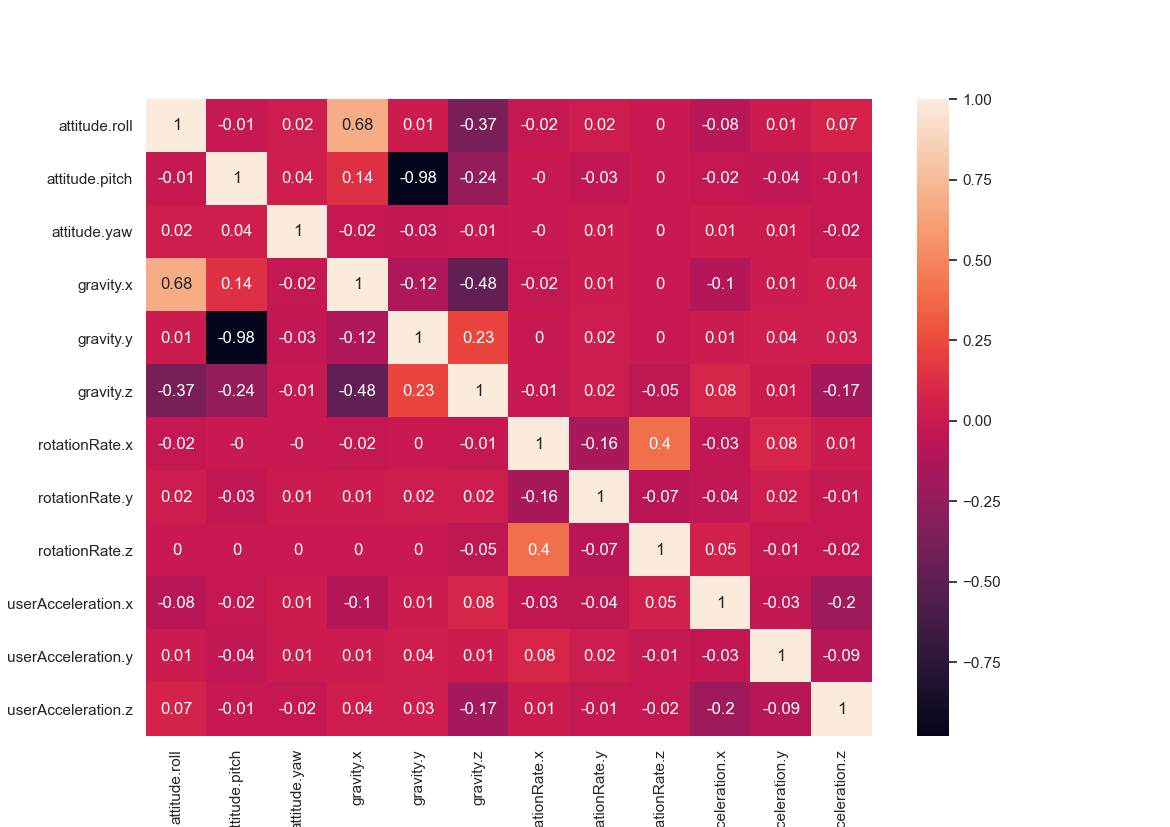
\includegraphics[scale=0.3]{correlation_matrix.png}
	\label{fig:correlation_matrix}
\end{figure}
\end{frame}

\end{document}